\documentclass{article}

% Language setting
% Replace `english' with e.g. `spanish' to change the document language
\usepackage[english]{babel}

% Set page size and margins
% Replace `letterpaper' with `a4paper' for UK/EU standard size
\usepackage[letterpaper,top=2cm,bottom=2cm,left=3cm,right=3cm,marginparwidth=1.75cm]{geometry}

% Useful packages
\usepackage{amsmath}
\usepackage{graphicx}
\usepackage[colorlinks=true, allcolors=blue]{hyperref}

\title{TDT4171 — Artificial Intelligence Methods \\ Assignment 5 - Making complex decisions}
\author{Erik Storås Sommer - 535006}
\date{February 2023}

\begin{document}
\maketitle
\setlength{\parindent}{0pt}

\section*{Exercise 1 - Decision Support System}

In this exercise, I have developed a decision support system to assist in choosing the most suitable cross-country skiing technique for a session.
This is a choice I often face when going on a ski session.
The choice is between whether I should choose to go classical technique or skating technique. The least desirable outcome is that there will be no session.

\subsection*{Modeling the system}

\begin{figure}[h]
    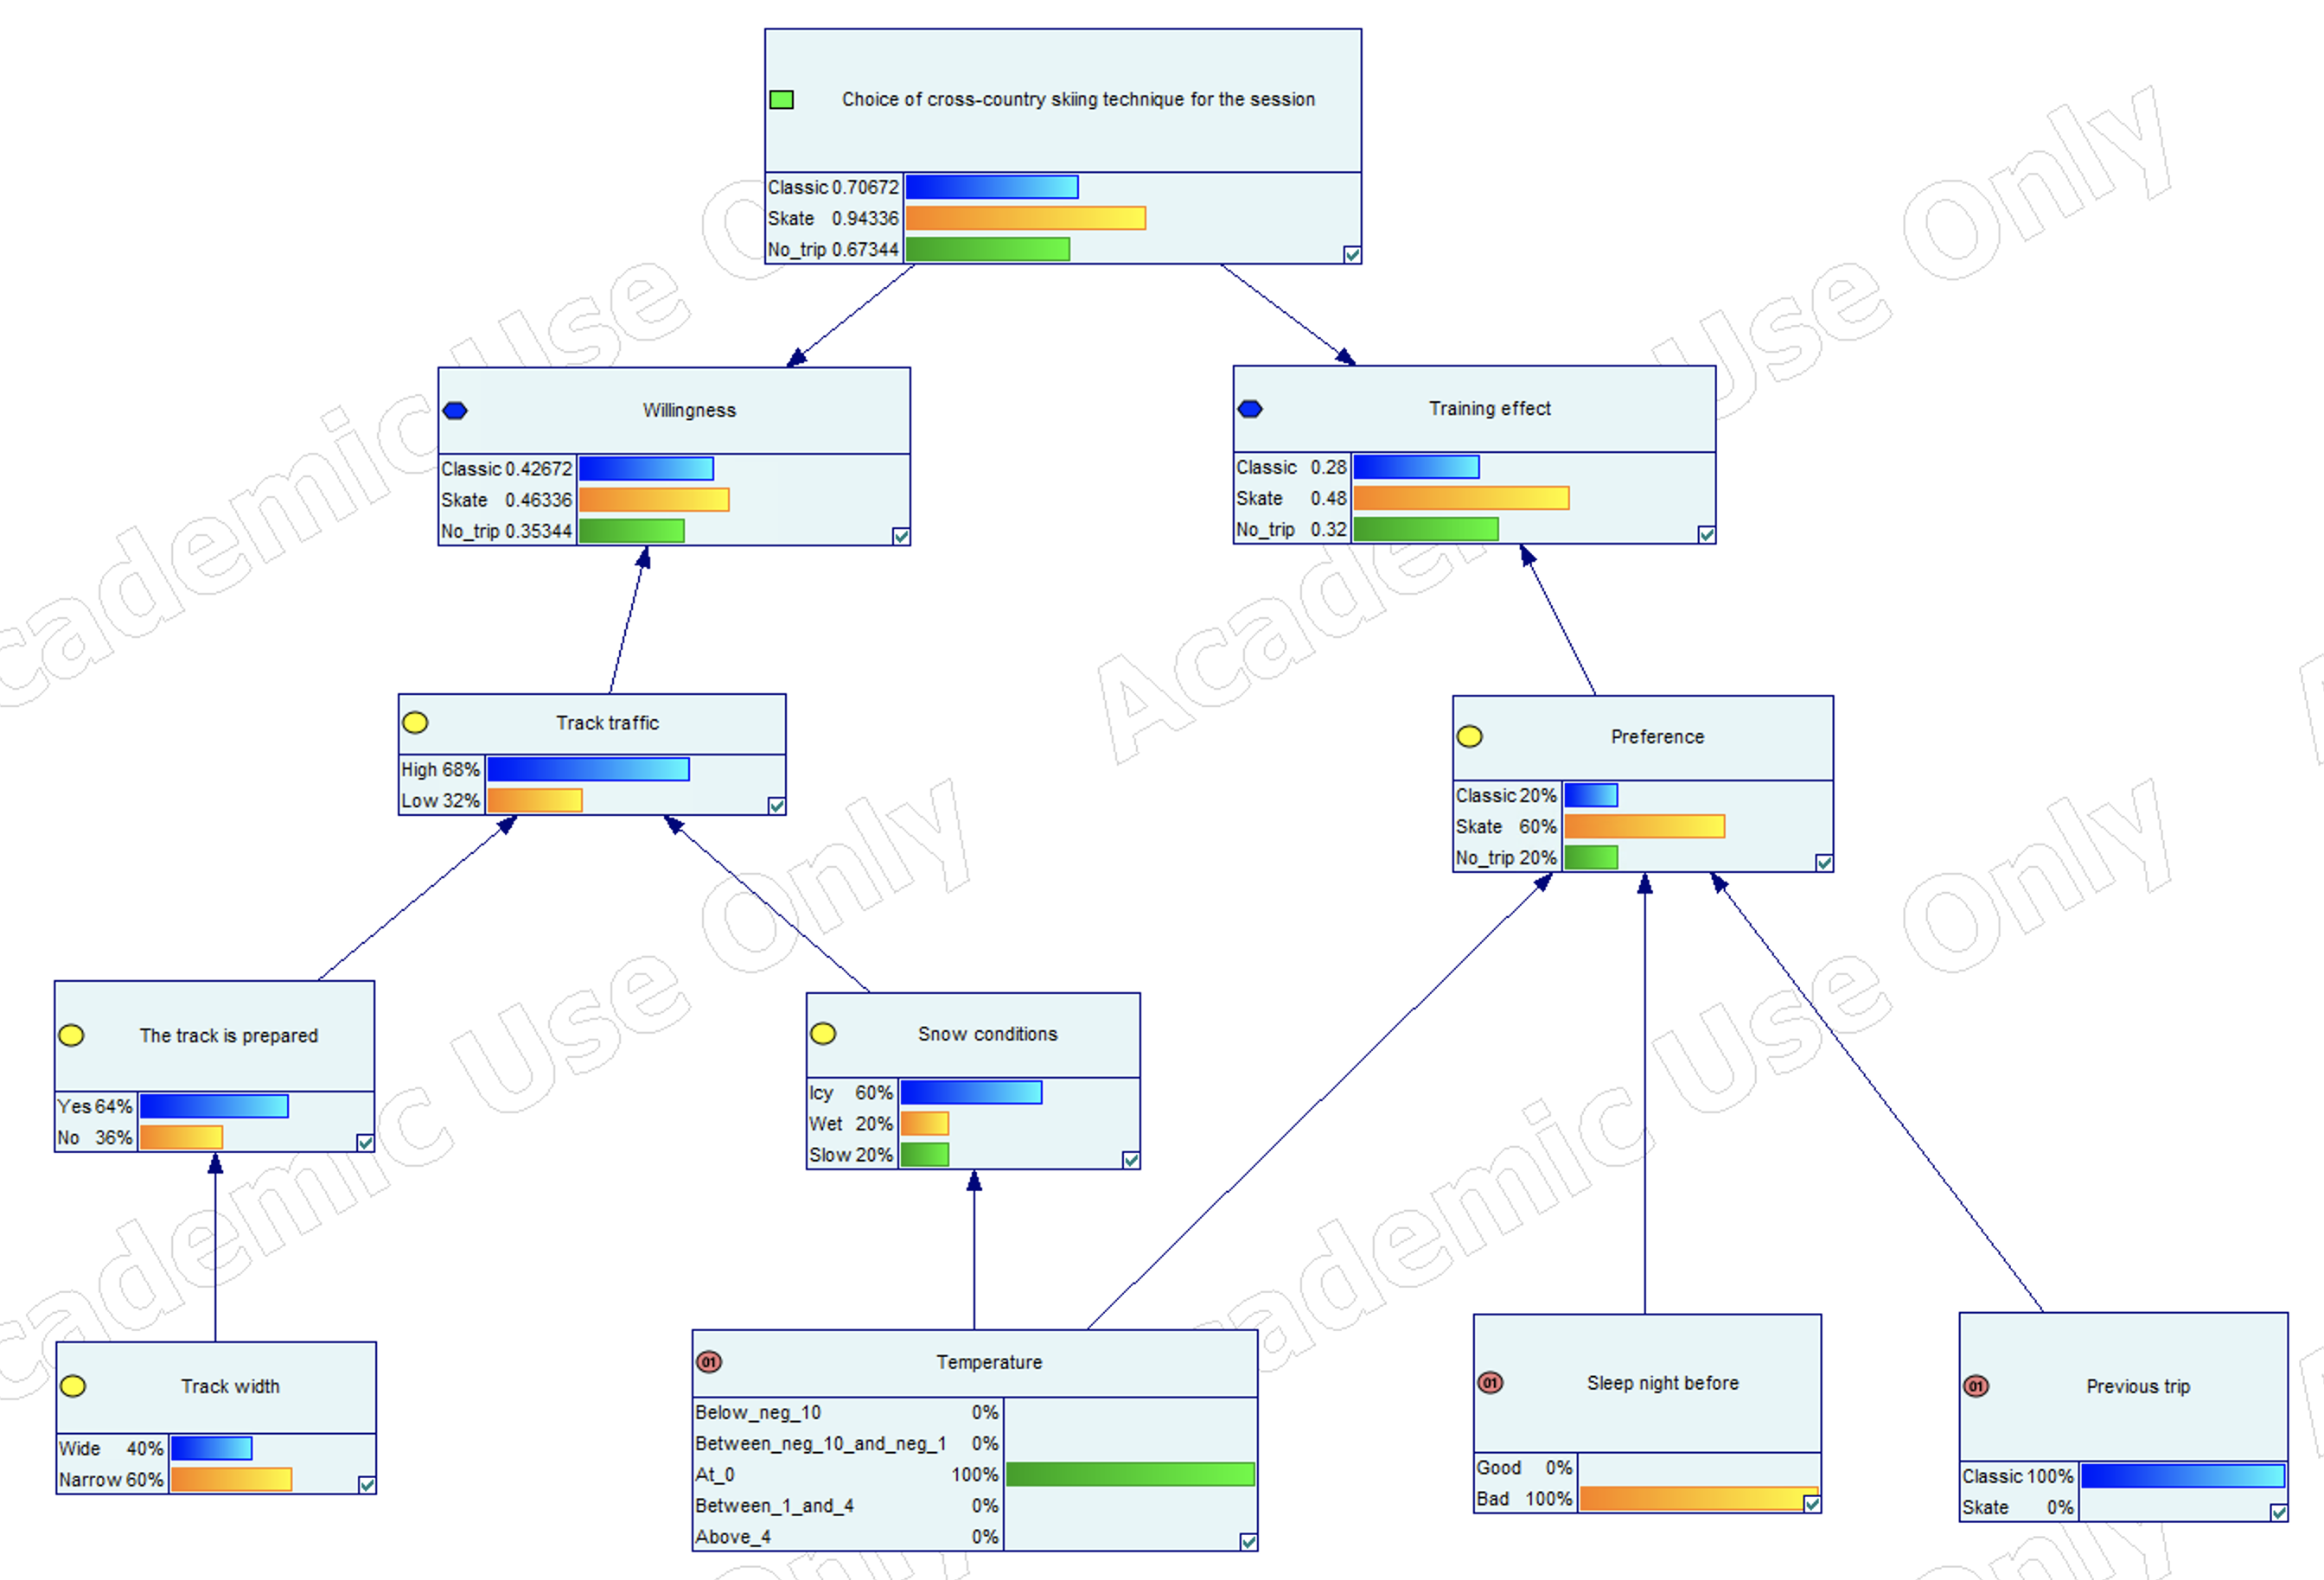
\includegraphics[width=\linewidth]{main_model.png}
    \caption{DSS}
    \label{fig:image1}
\end{figure}

Decision problem: Choice of cross-country skiing technique for the session.
\begin{itemize}
    \item Classic
    \item Skating
    \item No session (No trip)
\end{itemize}

Uncertan variables:
\begin{itemize}
    \item Track traffic
    \item The track is prepared
    \item Snow conditions
    \item Track width
    \item Preference
\end{itemize}

Certain variables:
\begin{itemize}
    \item Temperature
    \item Sleep night before
    \item Previous session (trip)
\end{itemize}

Utility functions:
\begin{itemize}
    \item Willingness
    \item Training effect
\end{itemize}

\subsection*{Probability tables}

Preference

\begin{figure}[h]
    \centering
    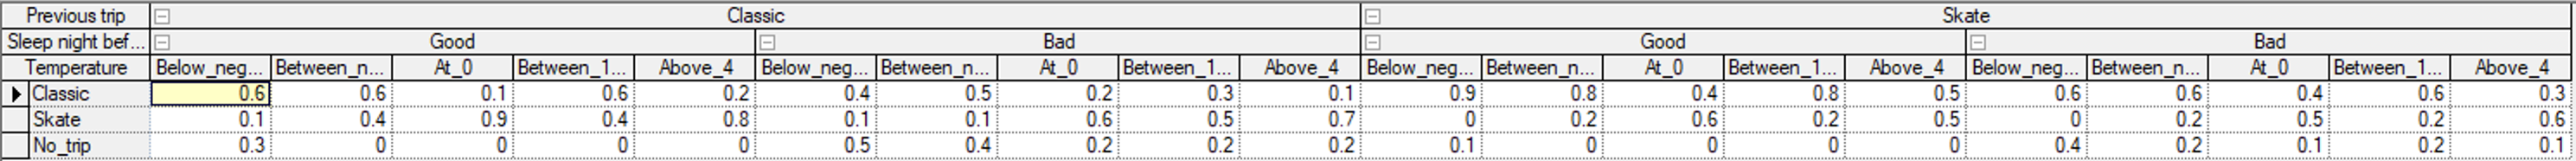
\includegraphics[width=\linewidth]{preference.png}
    \caption{Probability table for preference}
    \label{fig:image2}
\end{figure}

Snow conditions

\begin{figure}[h]
    \centering
    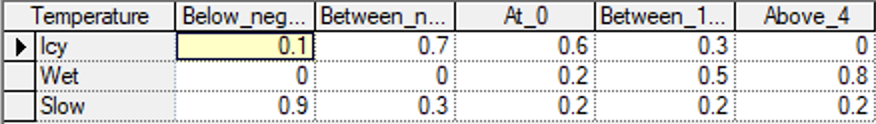
\includegraphics[width=\linewidth]{snow_conditions.png}
    \caption{Probability table for snow conditions}
    \label{fig:image3}
\end{figure}

Track traffic

\begin{figure}[h]
    \centering
    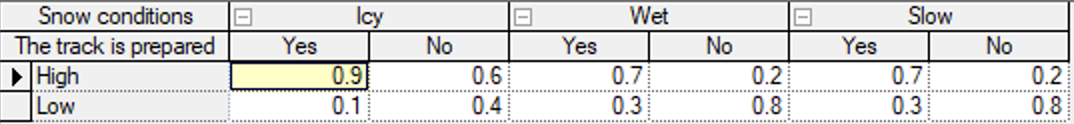
\includegraphics[width=\linewidth]{track_traffic.png}
    \caption{Probability table for track traffic}
    \label{fig:image4}
\end{figure}

\newpage

Willingness

\begin{figure}[h]
    \centering
    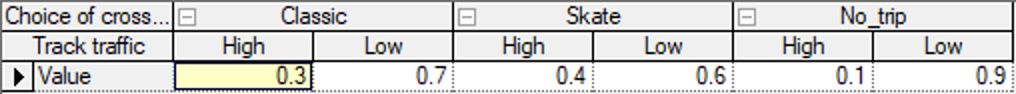
\includegraphics[width=\linewidth]{willingness.png}
    \caption{Probability table for willingness utility}
    \label{fig:image5}
\end{figure}

Training effect

\begin{figure}[h]
    \centering
    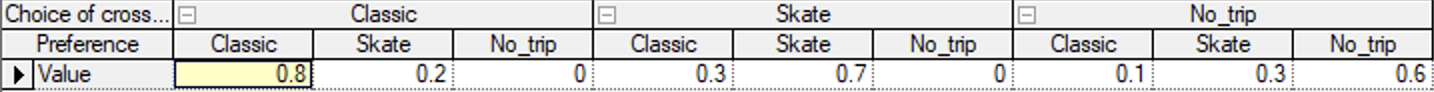
\includegraphics[width=\linewidth]{training_effect.png}
    \caption{Probability table for training effect utility}
    \label{fig:image6}
\end{figure}

\subsection*{Assumptions made in the model}

\begin{itemize}
    \item Both the willingness and training effect utility functions are dependant on the temperature.
    \item The willingness utility function is dependant on the track traffic, snow conditions and track width.
    \item The temperature is assumed to be constant for the entire session.
    \item The training effect utility function is dependant on the previous session, sleep the night before and temperature.
    \item The track width is conditionaly independant of snow conditions.
\end{itemize}

\subsection*{Results}

The system recommends skating, based on the following factors: good snow conditions, wide track width, high track traffic, most likely prepared track, previous session was classic, poor sleep the night before, and a temperature of 0 degrees.

\medskip

This result is reasonable given previous experiences.

\end{document}
